% !TEX encoding = UTF-8 Unicode

EPCON had an already built API which provided computer-aided diagnostics. This API accepted an x-ray photo encoded using base 64 and returned a diagnosis estimation. This is a computer-intensive process and it usually took between 10 to 40 seconds to respond. The point was to create a backend RESTful API to hide complexity and manage those heavy requests and then develop clients that would connect to this facade API.
\\ \\
This new API would also deliver features that were not present on the EPCON API, like user authentication, patient and screening data storage.

\\ \\
\begin{figure}[H]
	\centering
	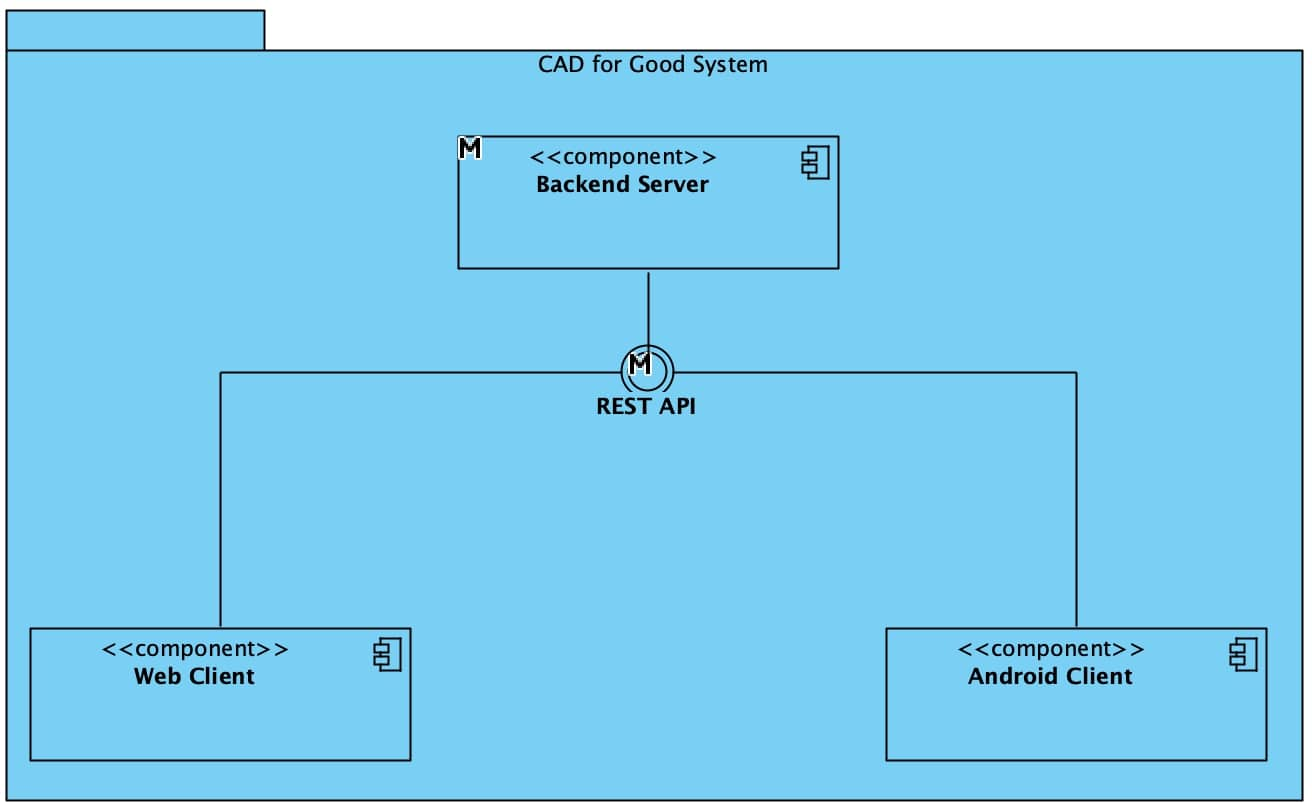
\includegraphics[width=1.0\linewidth]{pesti-report/images/global-system.jpg}
	\caption{System architecture}
	\label{fig:global-system}
\end{figure}
\\

The objective was to build clients with a focus on user-experience and which felt faster than directly requesting the EPCON servers.

\section{Implementation description}

To decide which technologies and frameworks we would use in order to develop the whole system we started by gathering information about the technical skills and previous experiences each of us had. We strongly thought about it and tried to not be influenced by the framework hype that exists nowadays. Many times during software development people put too much emphasis on the technology rather than the solution. We all agreed that we would go with the technologies that we felt comfortable with and not the ones that seemed better.
\\ \\
After this information gathering we decided to go with Node.js and Express for the back-end API, JavaScript and React for the web client and Kotlin and Java for the Android client.
\\
For designing the database schema we had to make some interesting decisions. One of the use cases required that the diagnose screening feature worked for both registered and unregistered users. For unregistered users the screening feature needed to be somehow connected to the specific device but EPCON also wanted to have the screening data persisted. To achieve this we added a device hash attribute to the Screening on the database schema and on the clients (web and Andorid) we would generate a unique hash and send it to the API on every diagnose screening request. This way we could merge all the local device screening with the ones persisted when an unregistered user finally decided to register.

\\ \\
\begin{figure}[H]
	\centering
	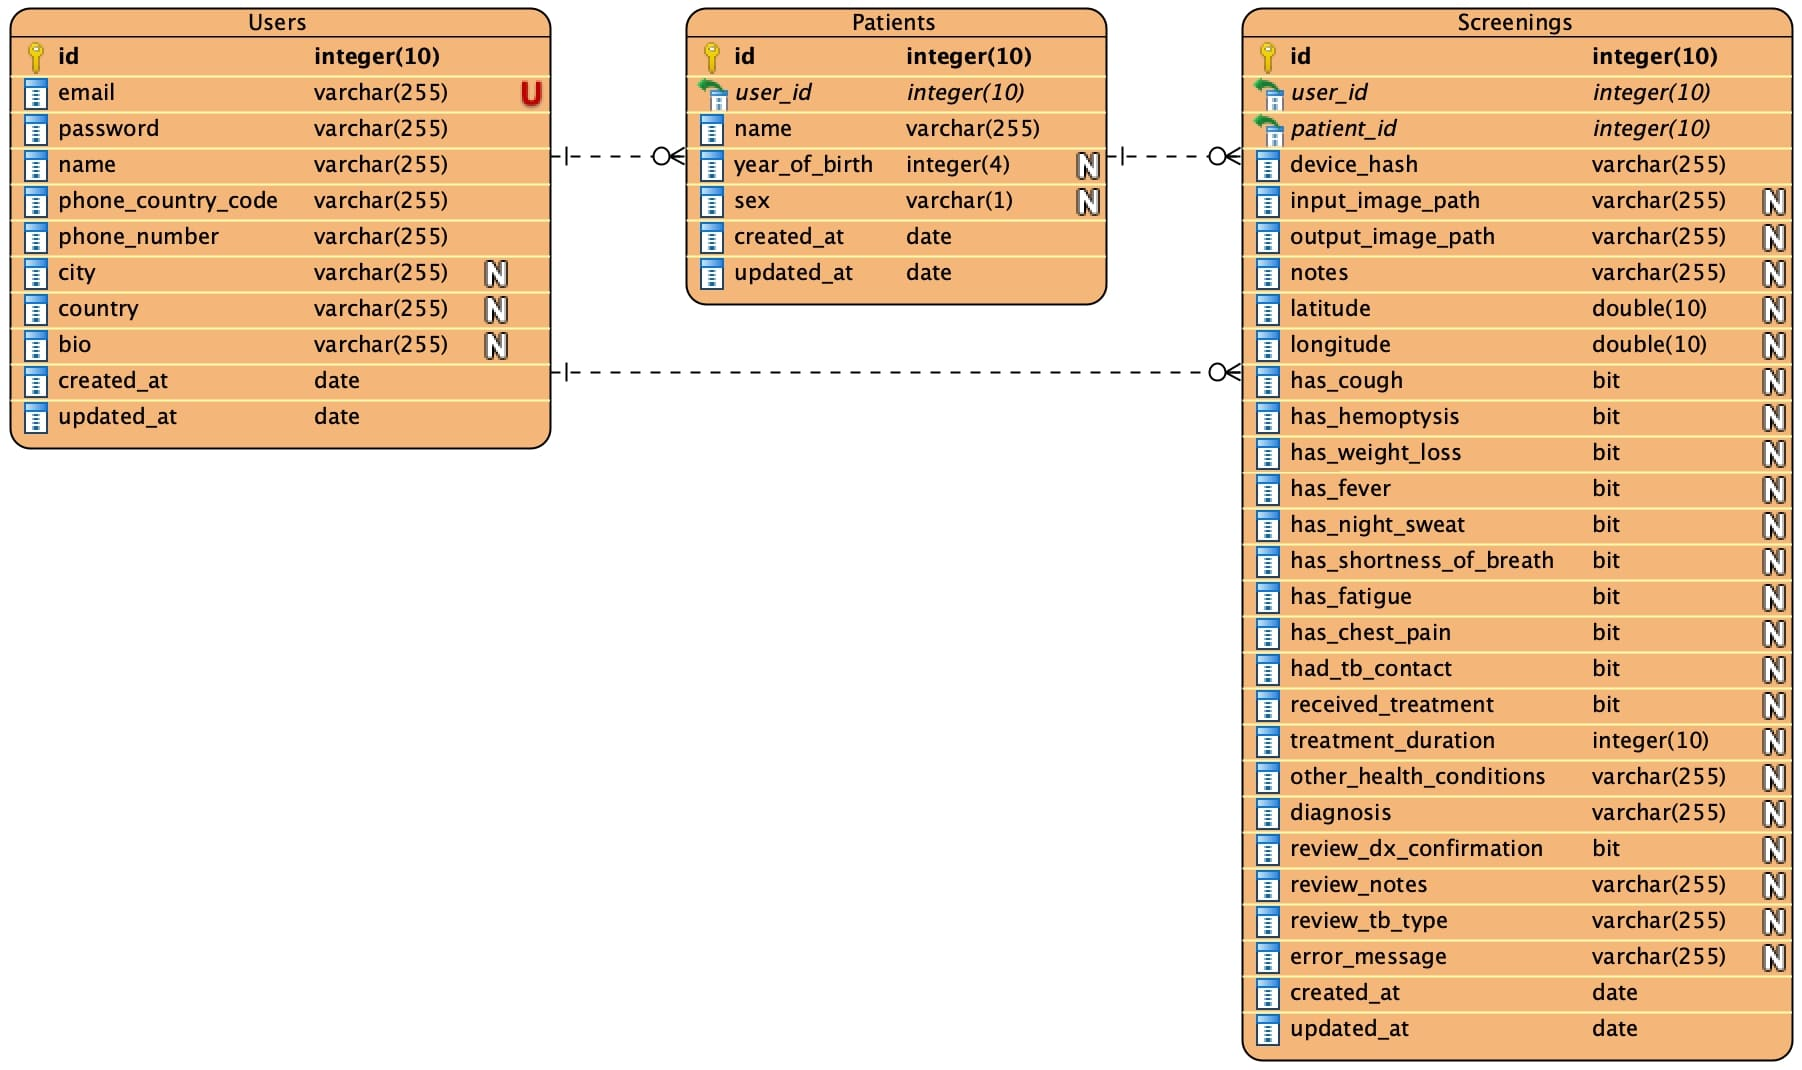
\includegraphics[width=1.0\linewidth]{pesti-report/images/database-schema.jpg}
	\caption{Database schema}
	\label{fig:database-schema}
\end{figure}
\\


\section{Backend architecture}

Our back-end was built using Node.js, a JavaScript run-time engine for server-side applications. To manage our API routes we used a popular Node.js framework named Express which made the endpoint development easier for us because of the framework API and nice online documentation.
\\ \\
We structured our code using different components that internally worked together. When a client would request our sever API the request would be caugth by our routes components, then it would pass by our middleware functions (different middlewares depending on the endpoint), then it would pass to our controllers and then, depending on the use case, hitting our database using our data access functions or generating some background service throught the use of events.


\\ \\
\begin{figure}[H]
	\centering
	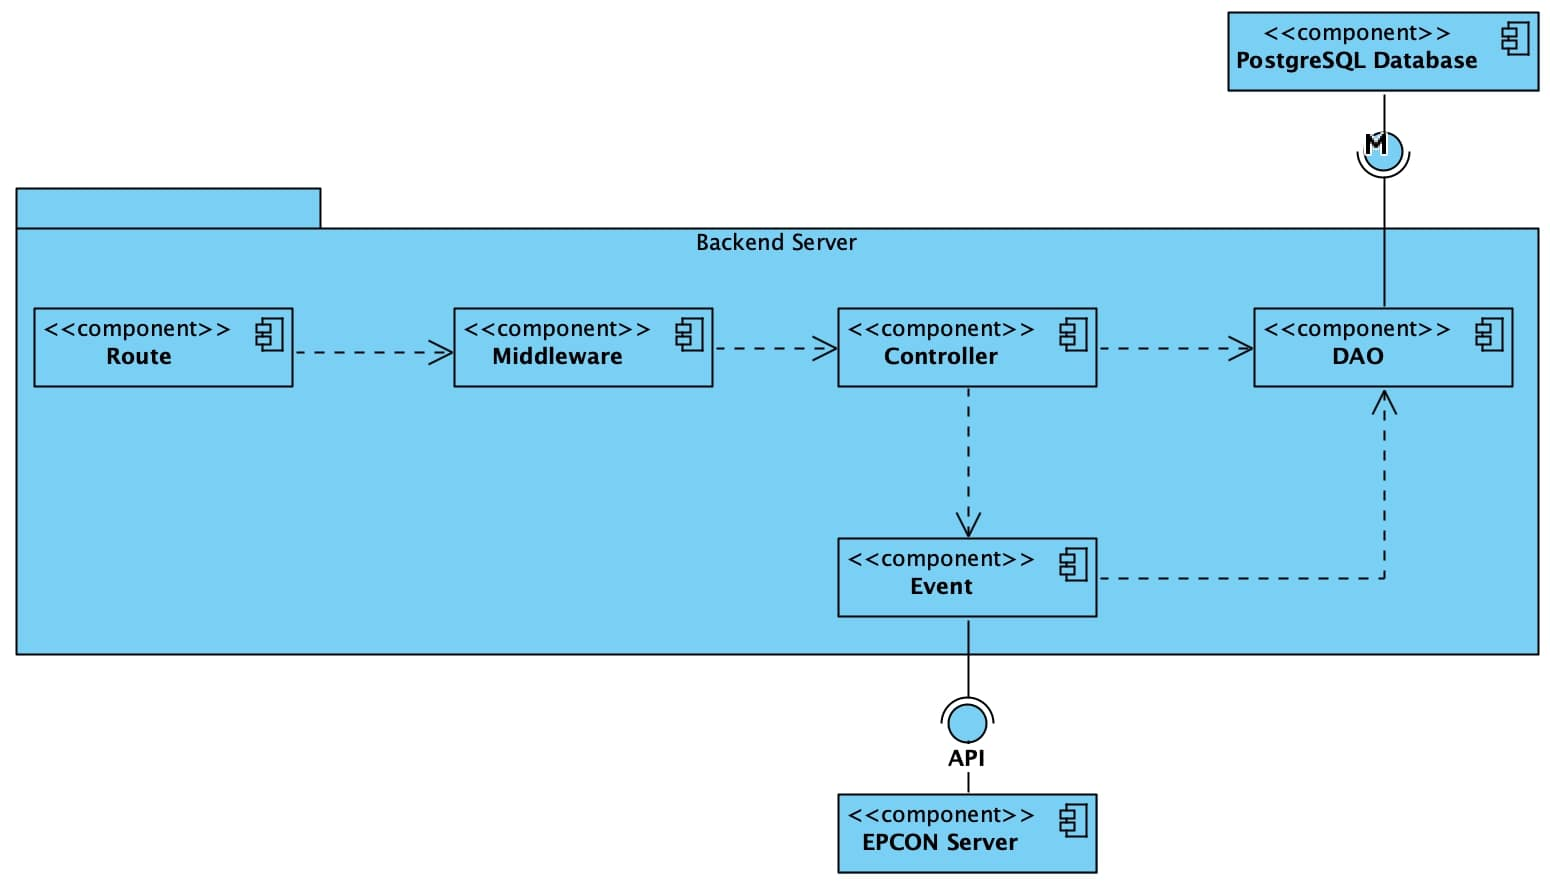
\includegraphics[width=1.0\linewidth]{pesti-report/images/backend-server-architecture.jpg}
	\caption{Backend server architecture}
	\label{fig:backend-server-architecture}
\end{figure}
\\

While designing and building this API, we had to make some interesting decisions. Here I will explain two of them in greater detail.

\subsection{User authentication}

To build our user authentication system with security on our minds we have created 2 different endpoints, one to register using email and password and another to login, also using email and password. When a user registers we check if the email address is already persisted in our database and if not we process to encrypt the password using a gold-standard open source password encryption npm module named bcrypt and then save the user on the database.
\\ \\
When the user logs in we compare the plain-text password to the encrypted one on the database using a bcrypt function and if it returns true we generate a JSON web token with the user id and return it to the client. Then client can decode the token but cannot modify it. This way, every time the client wants to request a private endpoint, it sends the token as a bearer token in the HTTP headers and the server can then decode the token, get the user id, and check if it was really that logged user who sent the request. This HTTP headers checking is done using our custom middleware functions.

\subsection{Background services}

One other challenge that we faced was the communication with EPCON API. To get diagnostics data from EPCON machine learning model, we have to first make a request to EPCON's authentication server, with a special username and login they provided for this project, get an authentication token (valid for 2 hours) from it, convert the multi-part-form JPEG or PNG image into base64 and then request an extremely slow-to-respond endpoint from EPCON bio-metrics server. This made the request to our endpoint extremely slow also, so we had to do it differently. When a user would submit a screening, it would save the initial details to the database and start a background service using a Node.js event. Then we would respond back to the client with the initial data stored about the screening, but with the diagnosis data still empty. And then, in the background service we would request the EPCON authentication server, get the token and then convert the images and request the bio-metrics server to get the diagnosis data. After that we would update that specific screening on the database.
\\ \\
After we updated the screening on the database we were thinking about using web-scokets to inform the user that the screening was updated with the diagnosis data, but, because of our lack of time, we did't yet implement this feature, so right now, we show the user information that says the screening is still processing and ask the user to refresh the page to fetch new data. We use this short polling technique while we don't have this web-socket feature proper implemented yet.


\section{Web client structure}

Our web application was written using JavaScript and React. We boostrapped our project using create-react-app which is a command line tool built by Facebook to people set up a modern React web app \cite{CreateReactApp}, and Bootstrap which is the world’s most popular front-end open source framework to quickly design and customize responsive mobile-first sites, featuring SASS variables and mixins, responsive grid system, extensive pre-built components, and powerful JavaScript plugins \cite{Bootstrap}.
\\ \\
The overall component schema of the web application can be seen in the image below.

\\ \\
\begin{figure}[H]
	\centering
	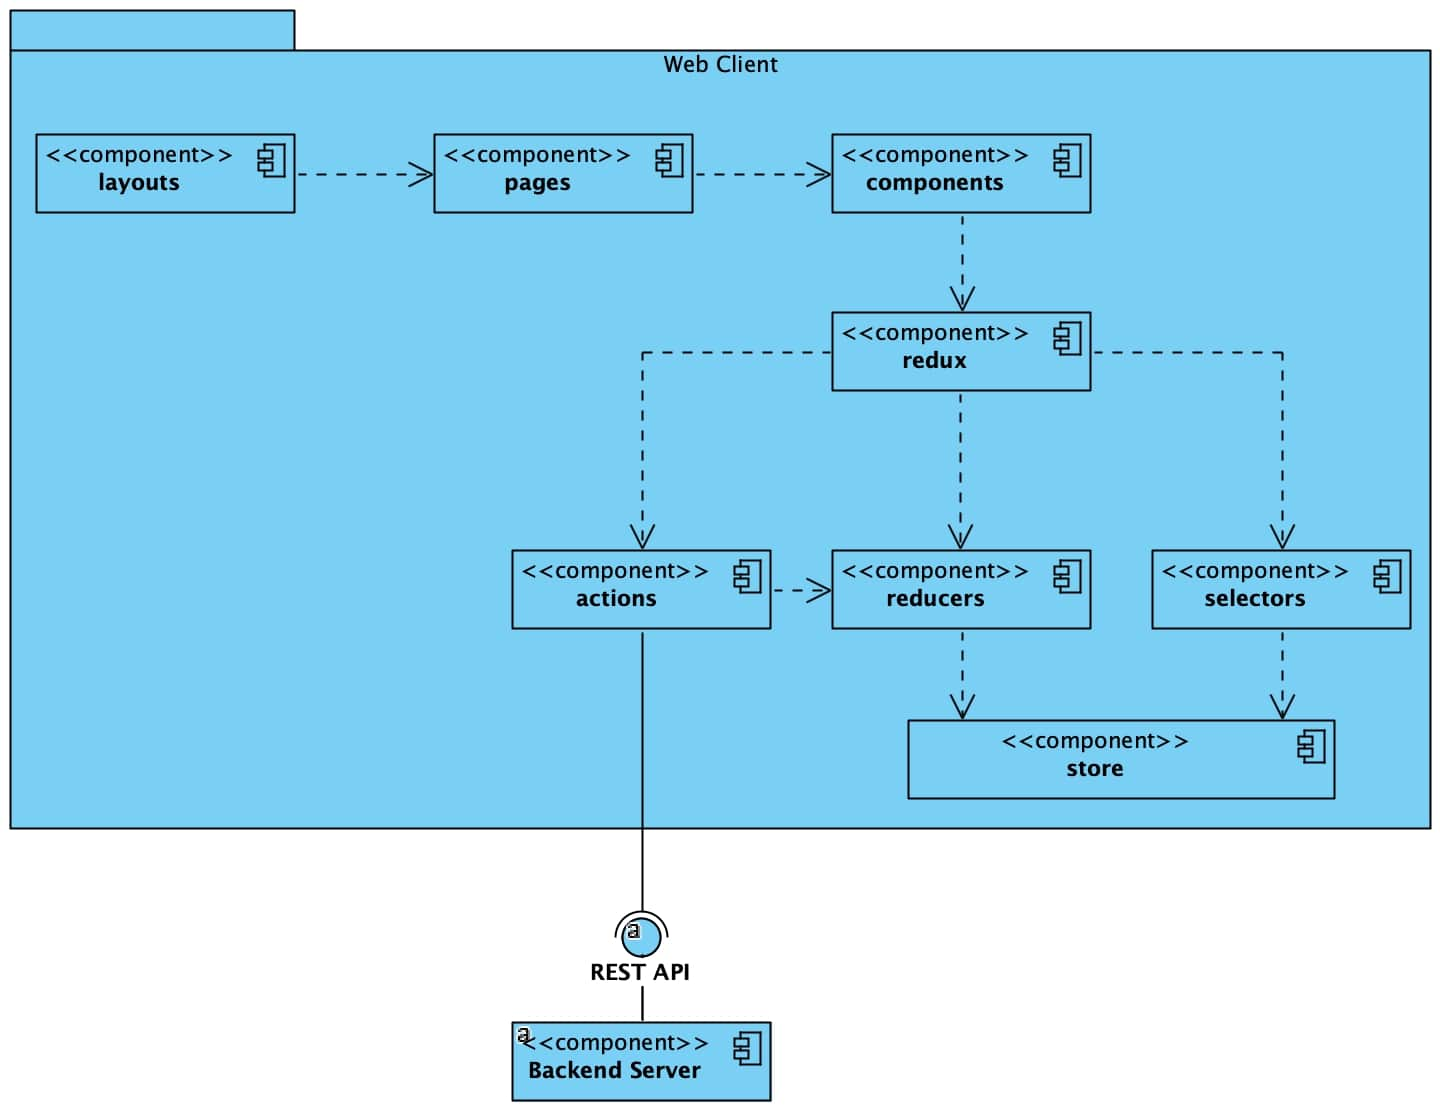
\includegraphics[width=1.0\linewidth]{pesti-report/images/web-client-structure.jpg}
	\caption{Web client structure}
	\label{fig:web-client-structure}
\end{figure}
\\

The visualization part is composed of pages, composed by a layout and many components.
\\ \\
If a component needs to post some data through the API of our backend server it needs to use our Redux layer. The component uses this layer by calling action functions, which are going to hit the API and call different action types which activate different reducers that will mutate the Redux store state.
\\ \\
If a component needs to fetch some data from the API it also needs to pass by the Redux layer, this time by using selector functions, which will return a specific piece of state to that component.
\\ \\
Below we can see a screenshot of our Redux store state at a given point in time. It holds information about the user profile, loading and error states and a memory cache of all the patients and screenings that were already fetched from the API.

\\ \\
\begin{figure}[H]
	\centering
	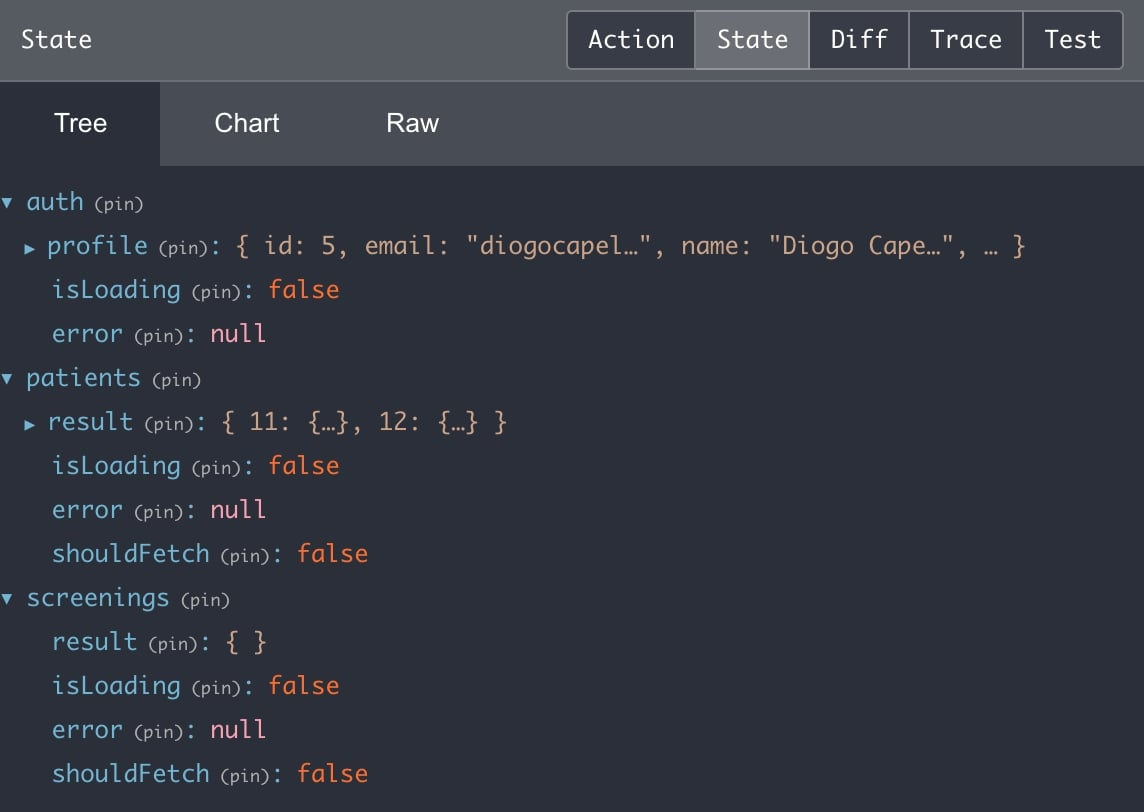
\includegraphics[width=1.0\linewidth]{pesti-report/images/redux-store.jpg}
	\caption{Redux store}
	\label{fig:redux-store}
\end{figure}
\\

To style the website to match EPCON design needs we decided to use a SCSS, a CSS tool that give us more options when writing styles for our layouts and components.
\\ \\
In the figure below we can see a screenshot of the homepage of the web application.

\\ \\
\begin{figure}[H]
	\centering
	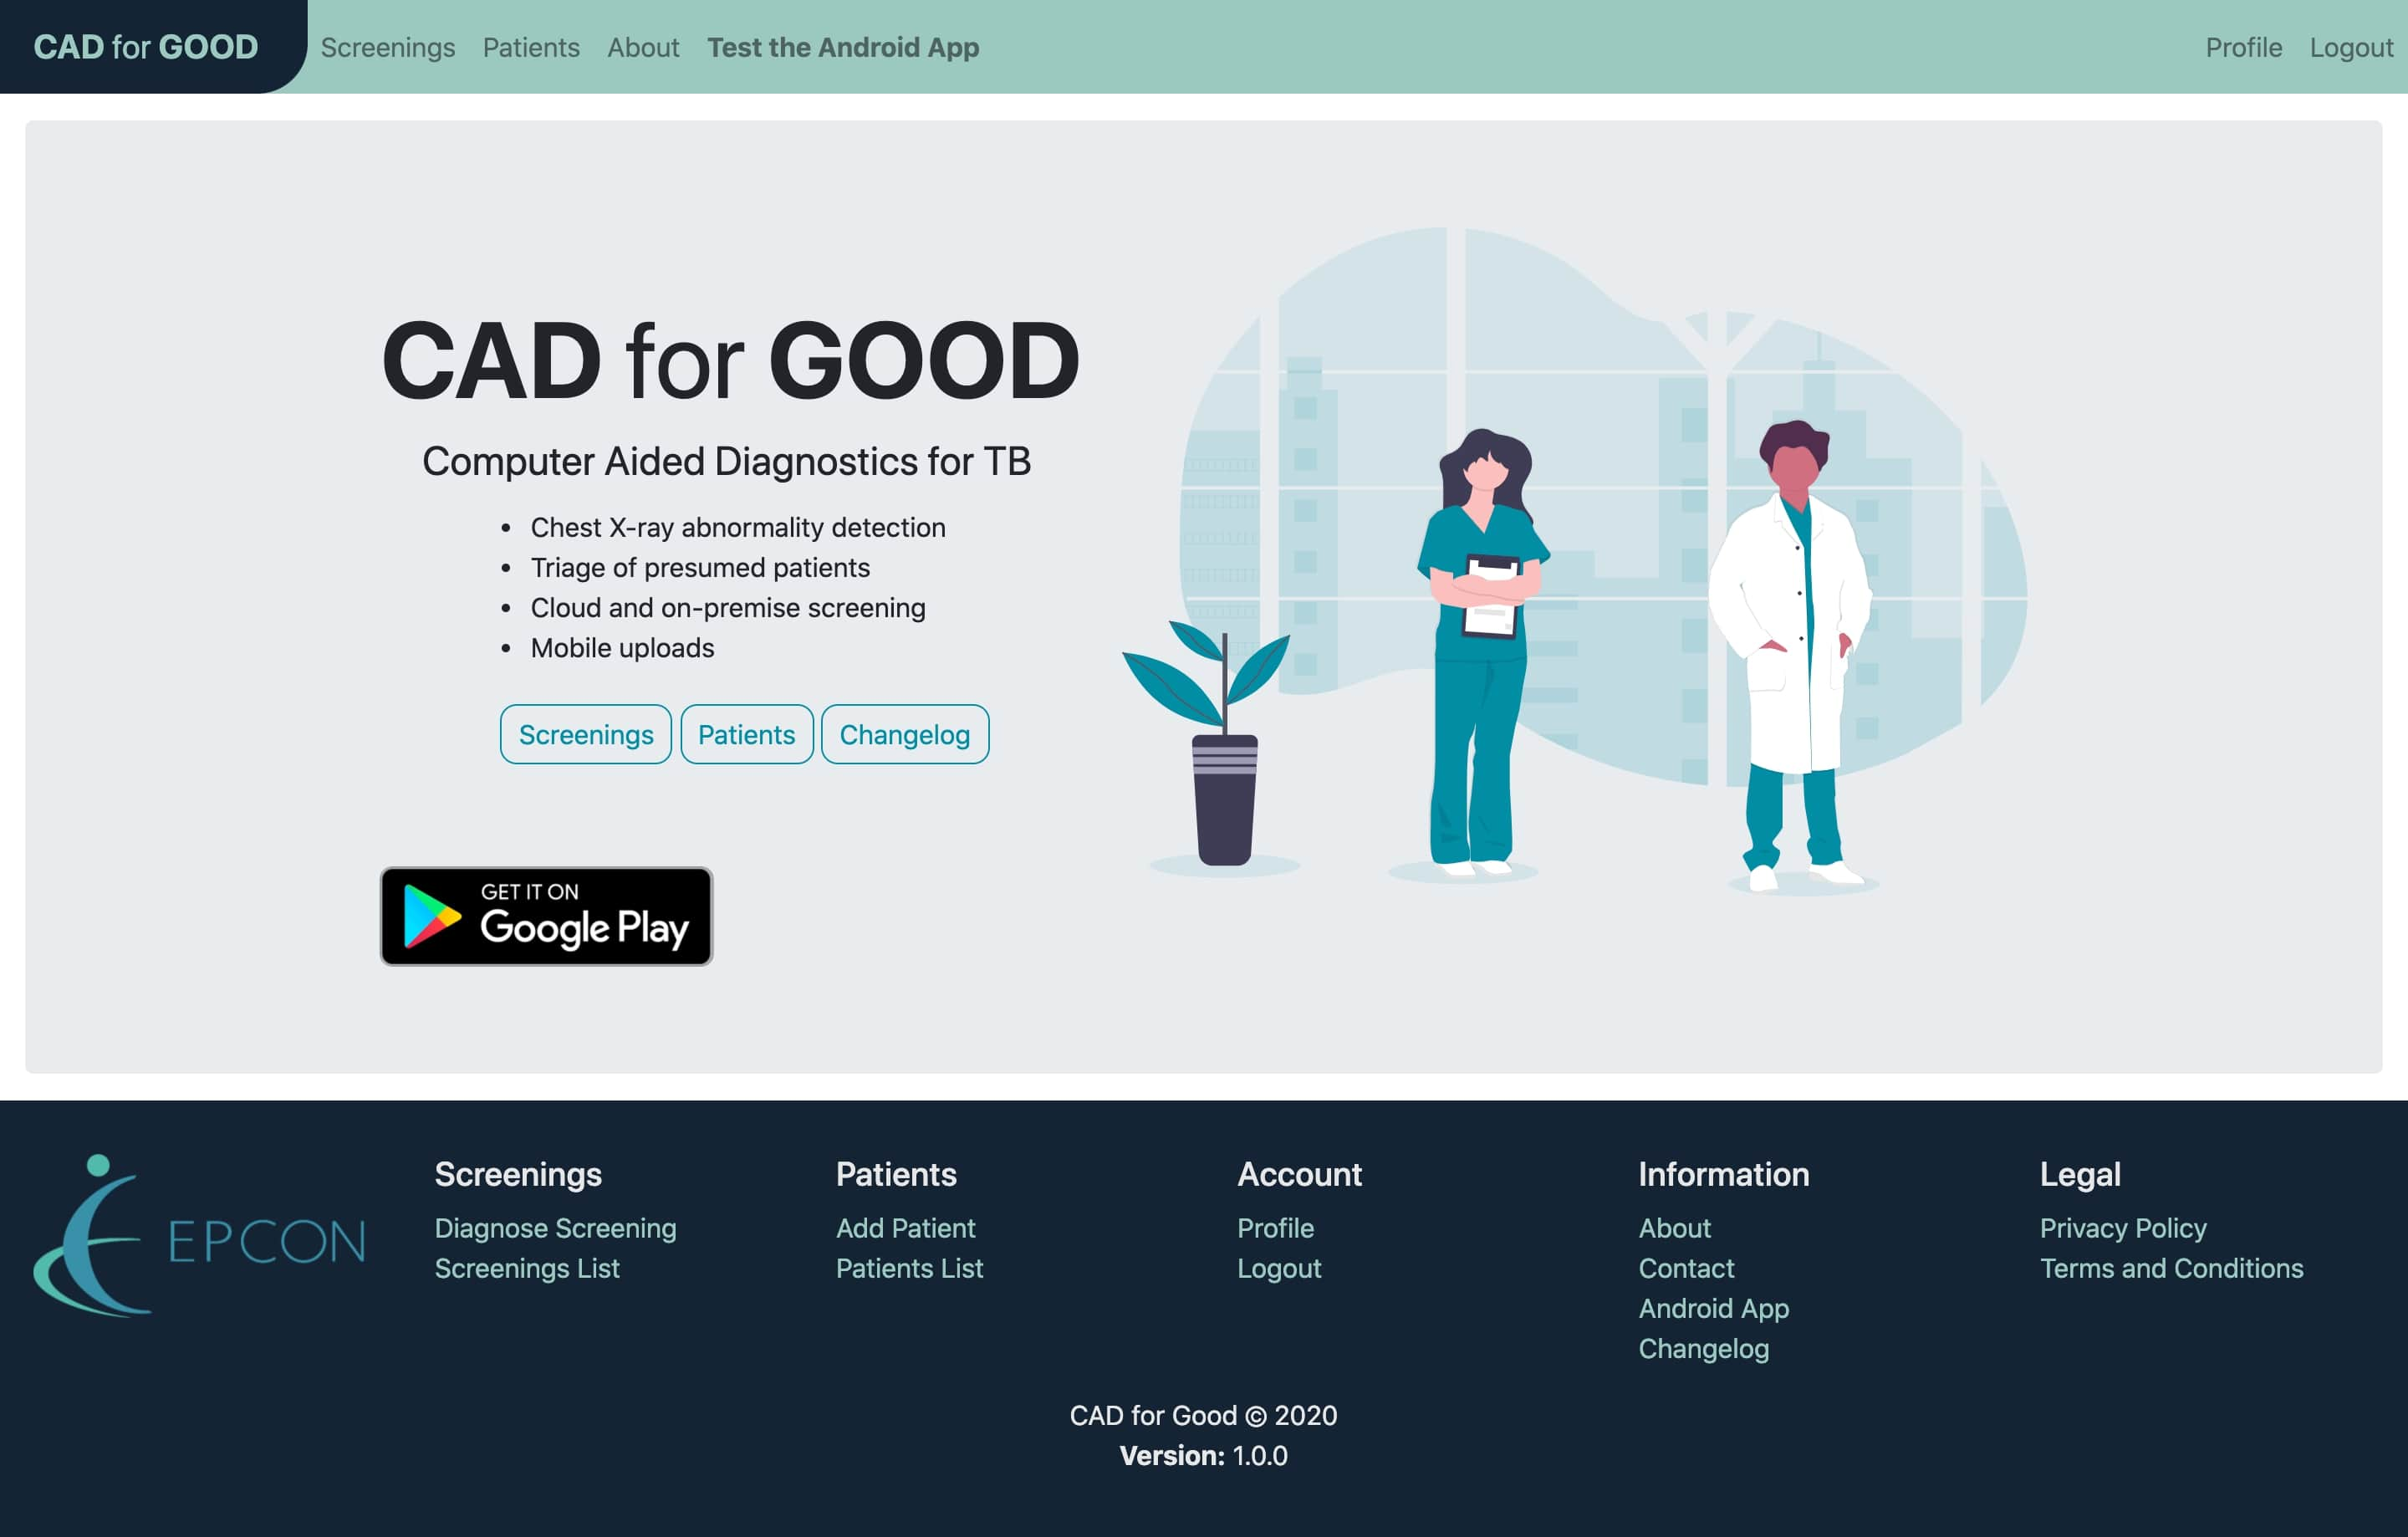
\includegraphics[width=1.0\linewidth]{pesti-report/images/web-client-screenshot-homepage.jpg}
	\caption{Homepage of the web application}
	\label{fig:web-client-screenshot-homepage}
\end{figure}
\\

The screening process starts by the client generating an unique device hash so every request do diagnose a screening can be traced back to the device.

\\ \\
\begin{figure}[H]
	\centering
	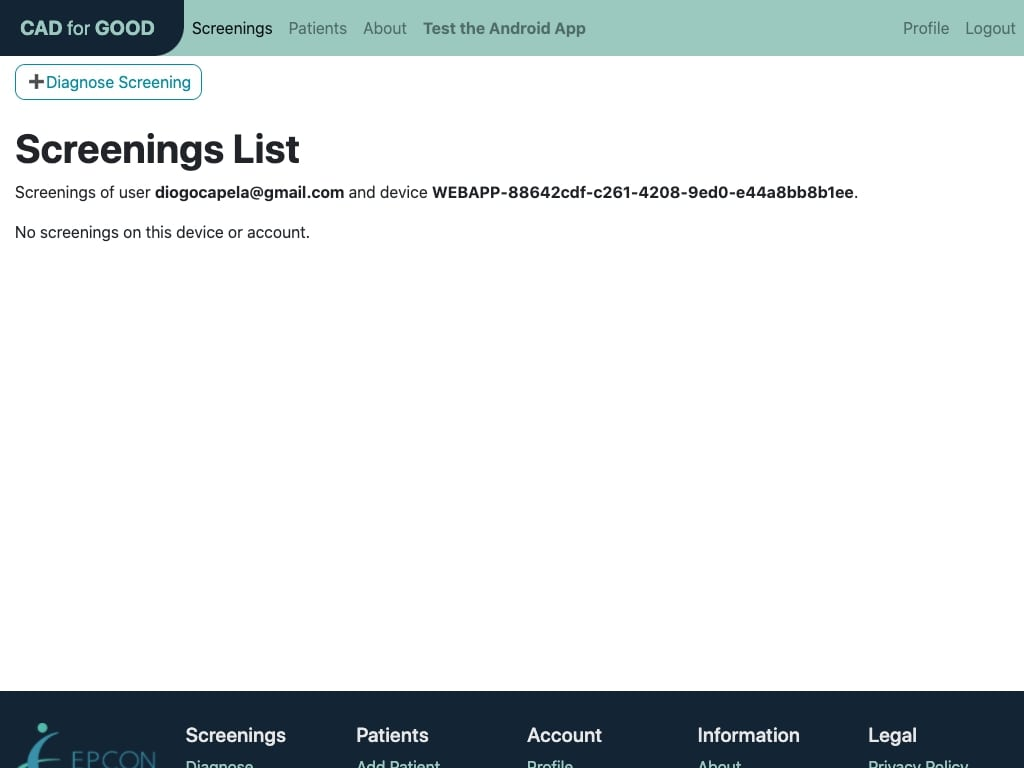
\includegraphics[width=1.0\linewidth]{pesti-report/images/web-client-screenshot-screenings-01.jpg}
	\caption{Empty screenings list}
	\label{fig:web-client-screenshot-screenings-01}
\end{figure}
\\

After we click on diagnose screening we are taken to a page where we can upload the X-ray picture and fill all the symptoms and additional details.

\\ \\
\begin{figure}[H]
	\centering
	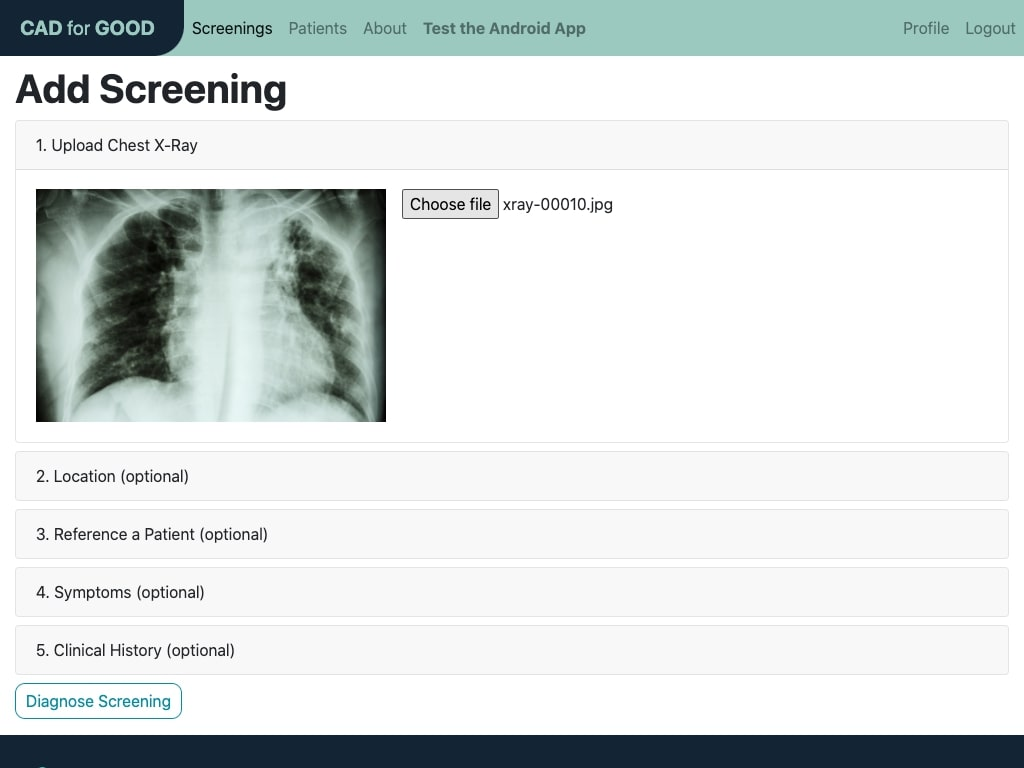
\includegraphics[width=1.0\linewidth]{pesti-report/images/web-client-screenshot-screenings-02.jpg}
	\caption{Submit a screening page}
	\label{fig:web-client-screenshot-screenings-02}
\end{figure}
\\

When we submit a screening the server is running it as a background service, so we should wait on the client side for it to be completed. After the screening has diagnostic data from the back-end we can view it in the screening details page you can see below:

\\ \\
\begin{figure}[H]
	\centering
	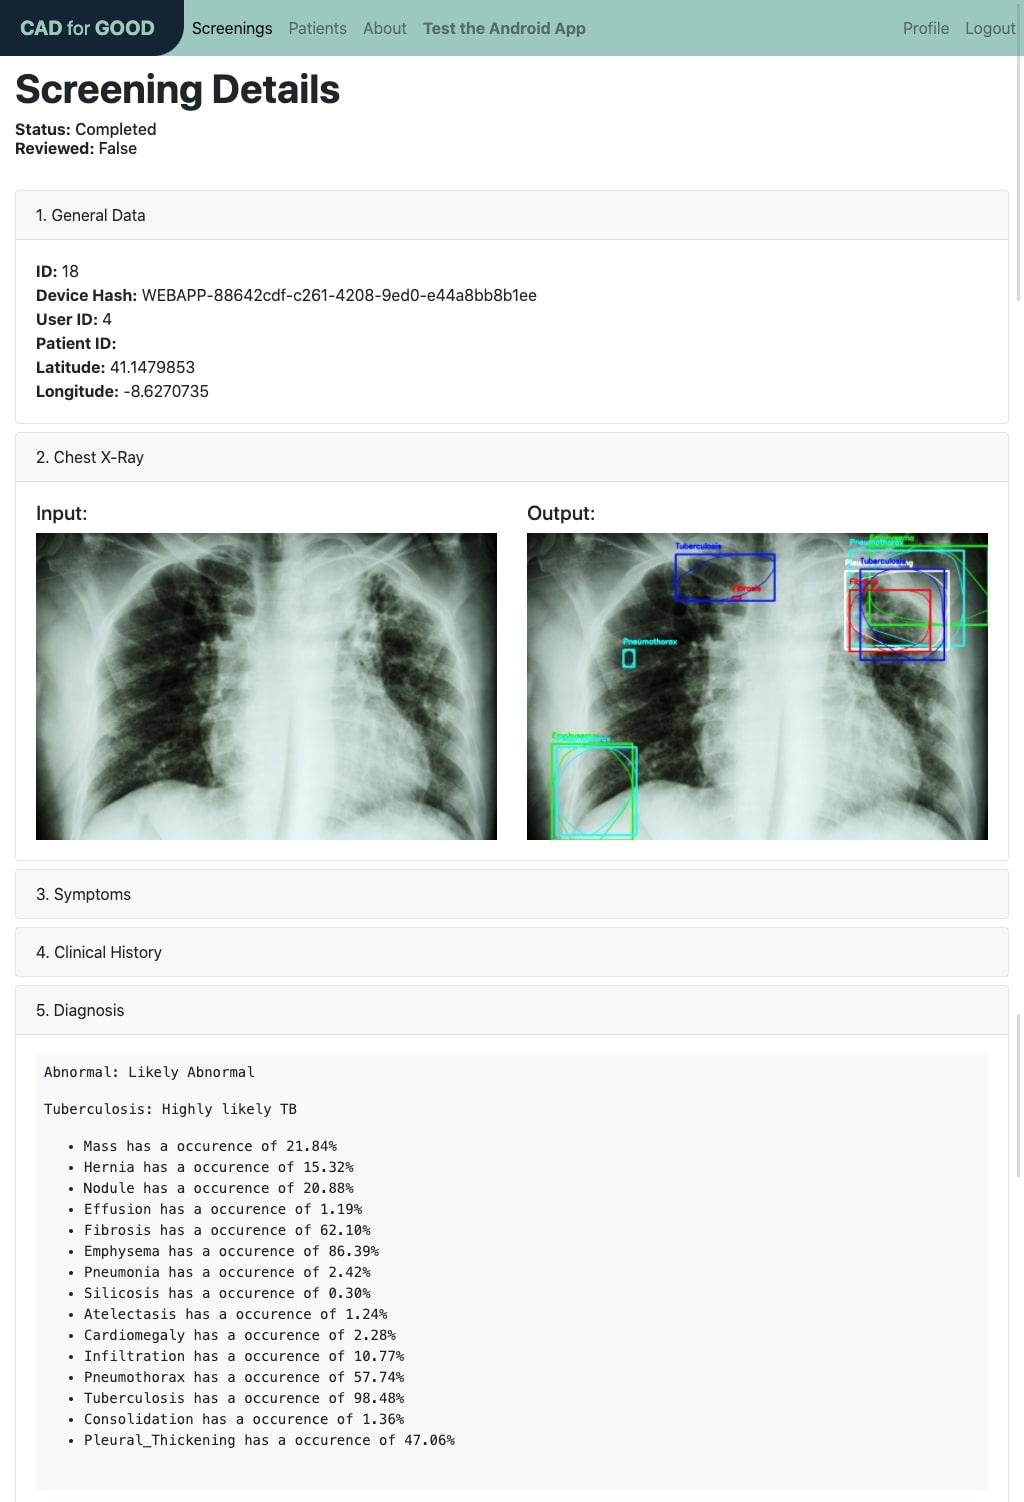
\includegraphics[width=1.0\linewidth]{pesti-report/images/web-client-screenshot-screenings-04.jpg}
	\caption{Screening details page}
	\label{fig:web-client-screenshot-screenings-04}
\end{figure}
\\



\section{Android client structure}

To build the Android client we use the standard development tools: Android Studio and the JDK for Android. We decided to build a native application because most of our team was familiar with Java, the programming language used by Android Studio and the Android API.
\\ \\
We divided our components into layouts, composed by activities and fragments, both of them with logic glued to the respective controllers. And then this controllers would connect to our repositories which saved data locally using a SQLite database, or communicated directly with out back-end API.

\\ \\
\begin{figure}[H]
	\centering
	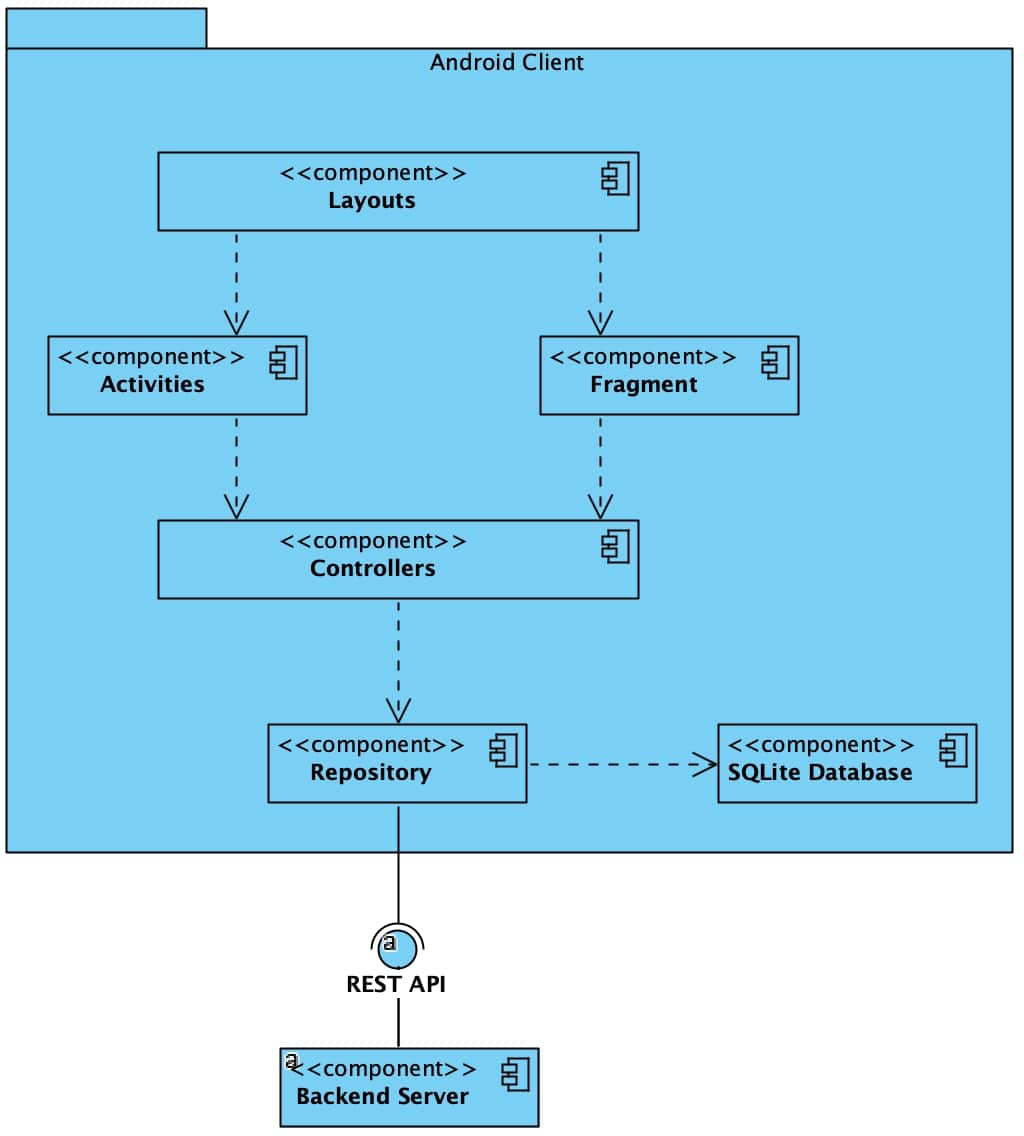
\includegraphics[width=1.0\linewidth]{pesti-report/images/android-client-structure.jpg}
	\caption{Android client structure}
	\label{fig:android-client-structure}
\end{figure}
\\

Below are some screenshots of the authentication layout we have at the time of this report.

\\ \\
\begin{figure}[H]
	\centering
	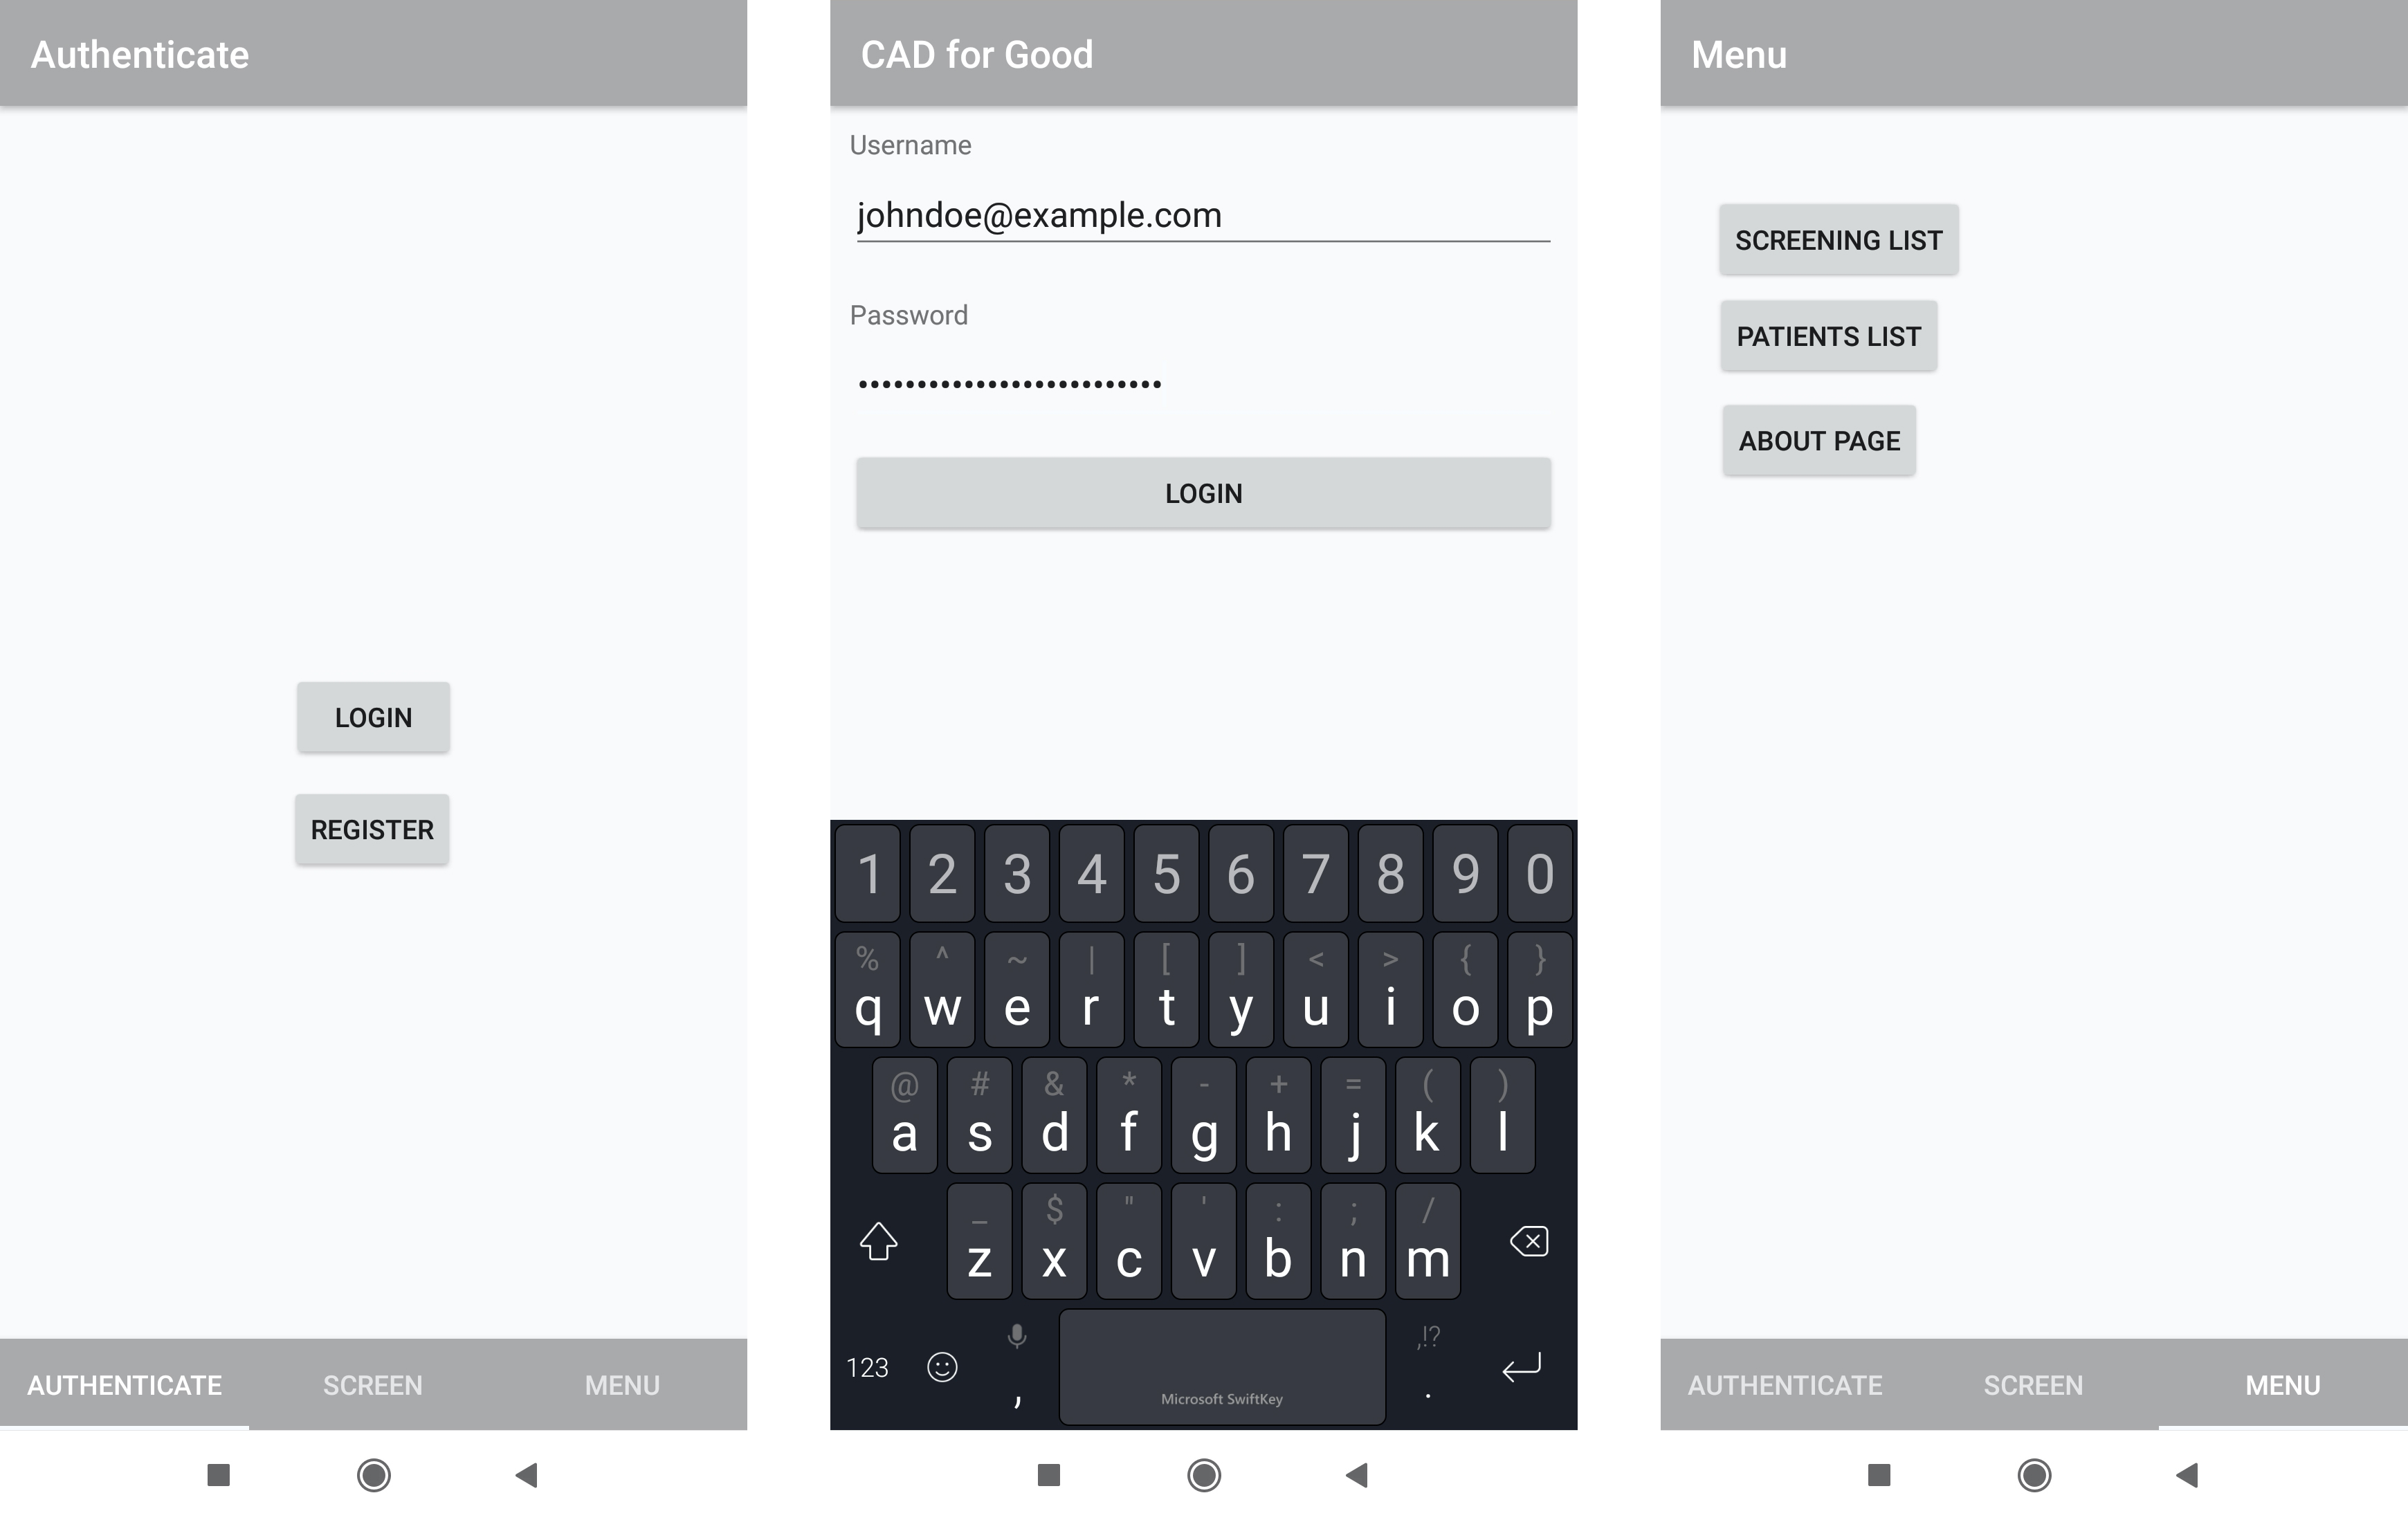
\includegraphics[width=1.0\linewidth]{pesti-report/images/android-client-screenshot-authentication.jpg}
	\caption{Android client authentication}
	\label{fig:android-client-authentication}
\end{figure}
\\

And below you can find the MVP layout for the screening submission process on our mobile app.

\\ \\
\begin{figure}[H]
	\centering
	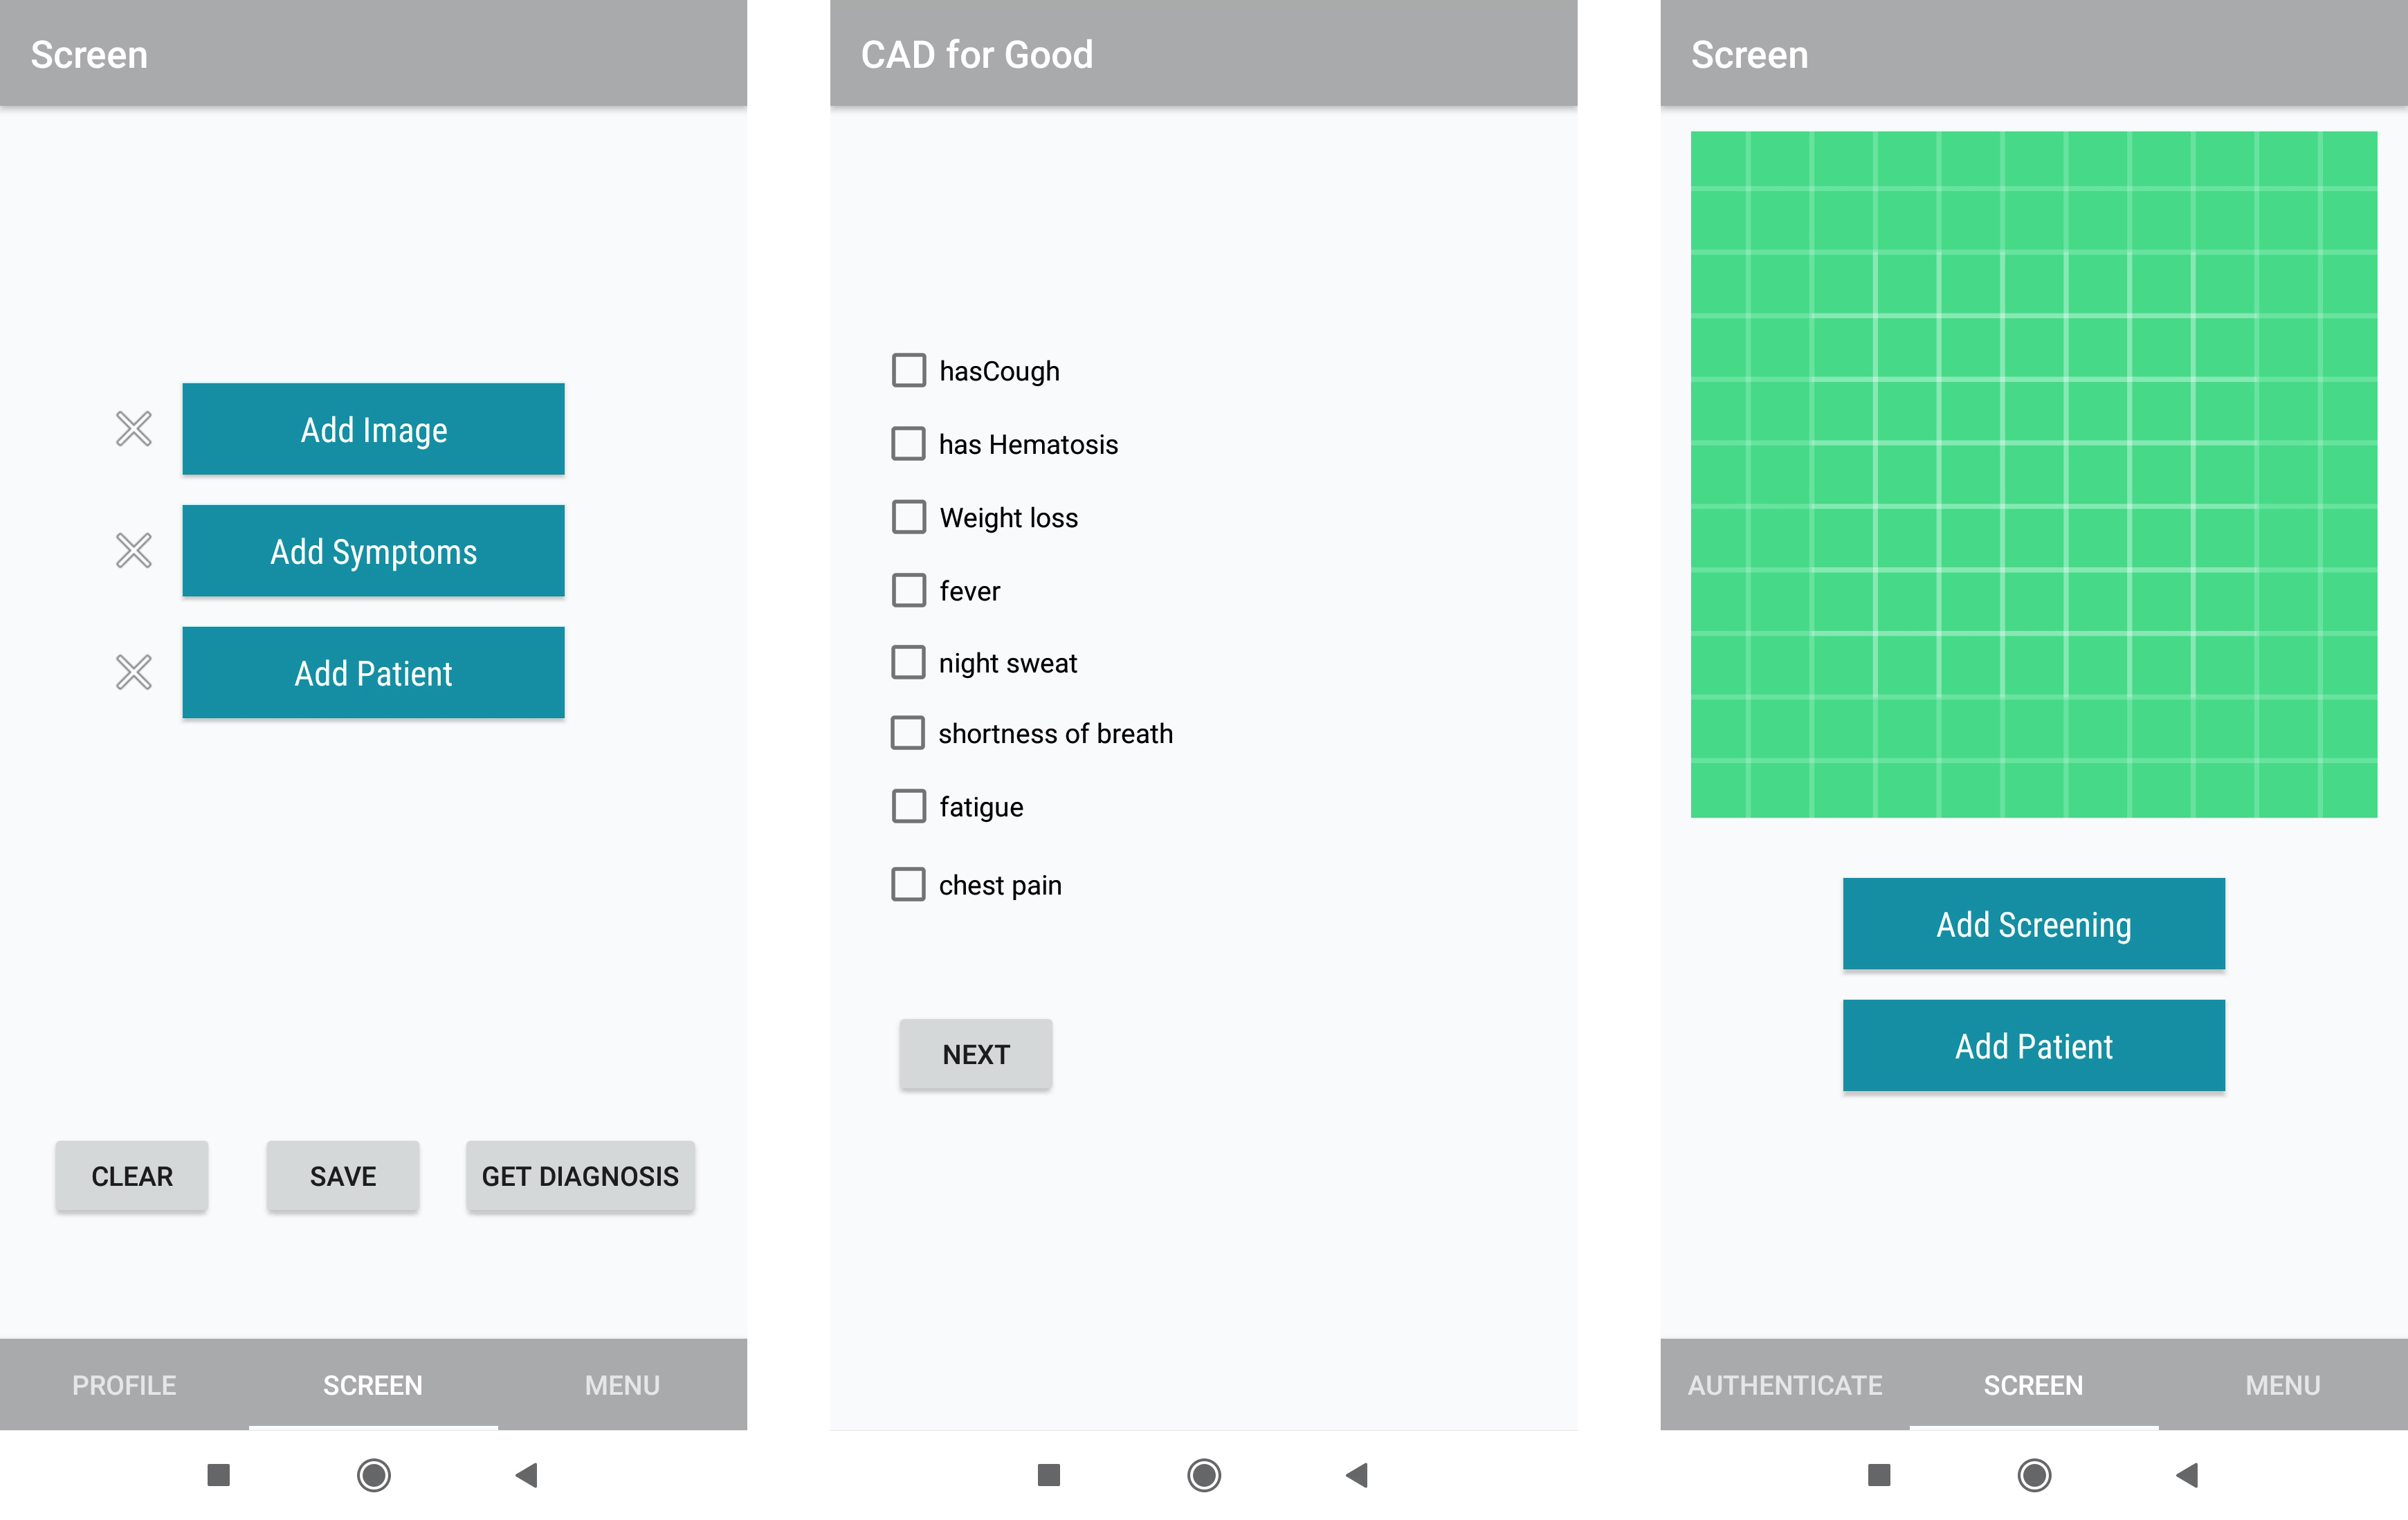
\includegraphics[width=1.0\linewidth]{pesti-report/images/android-client-screenshot-screen.jpg}
	\caption{Submit a screening using the Android app}
	\label{fig:android-client-screen}
\end{figure}
\\




\section{Tests}

We believe that we can only make sure that our code works if we test it. In this way, we have written unit tests for most of our API endpoints, where we would tests success cases and also error cases.
\\ \\
After some discussion about it, we decided to test only the back-end server and to not do front-end testing in our web and Android clients. We did't had the needed time to spend writting tests for all of our three components, so we decided to do it for the most important one, which was the back-end API. Below you can view a screenshot of some of the unit tests we wrote:


\\ \\
\begin{figure}[H]
	\centering
	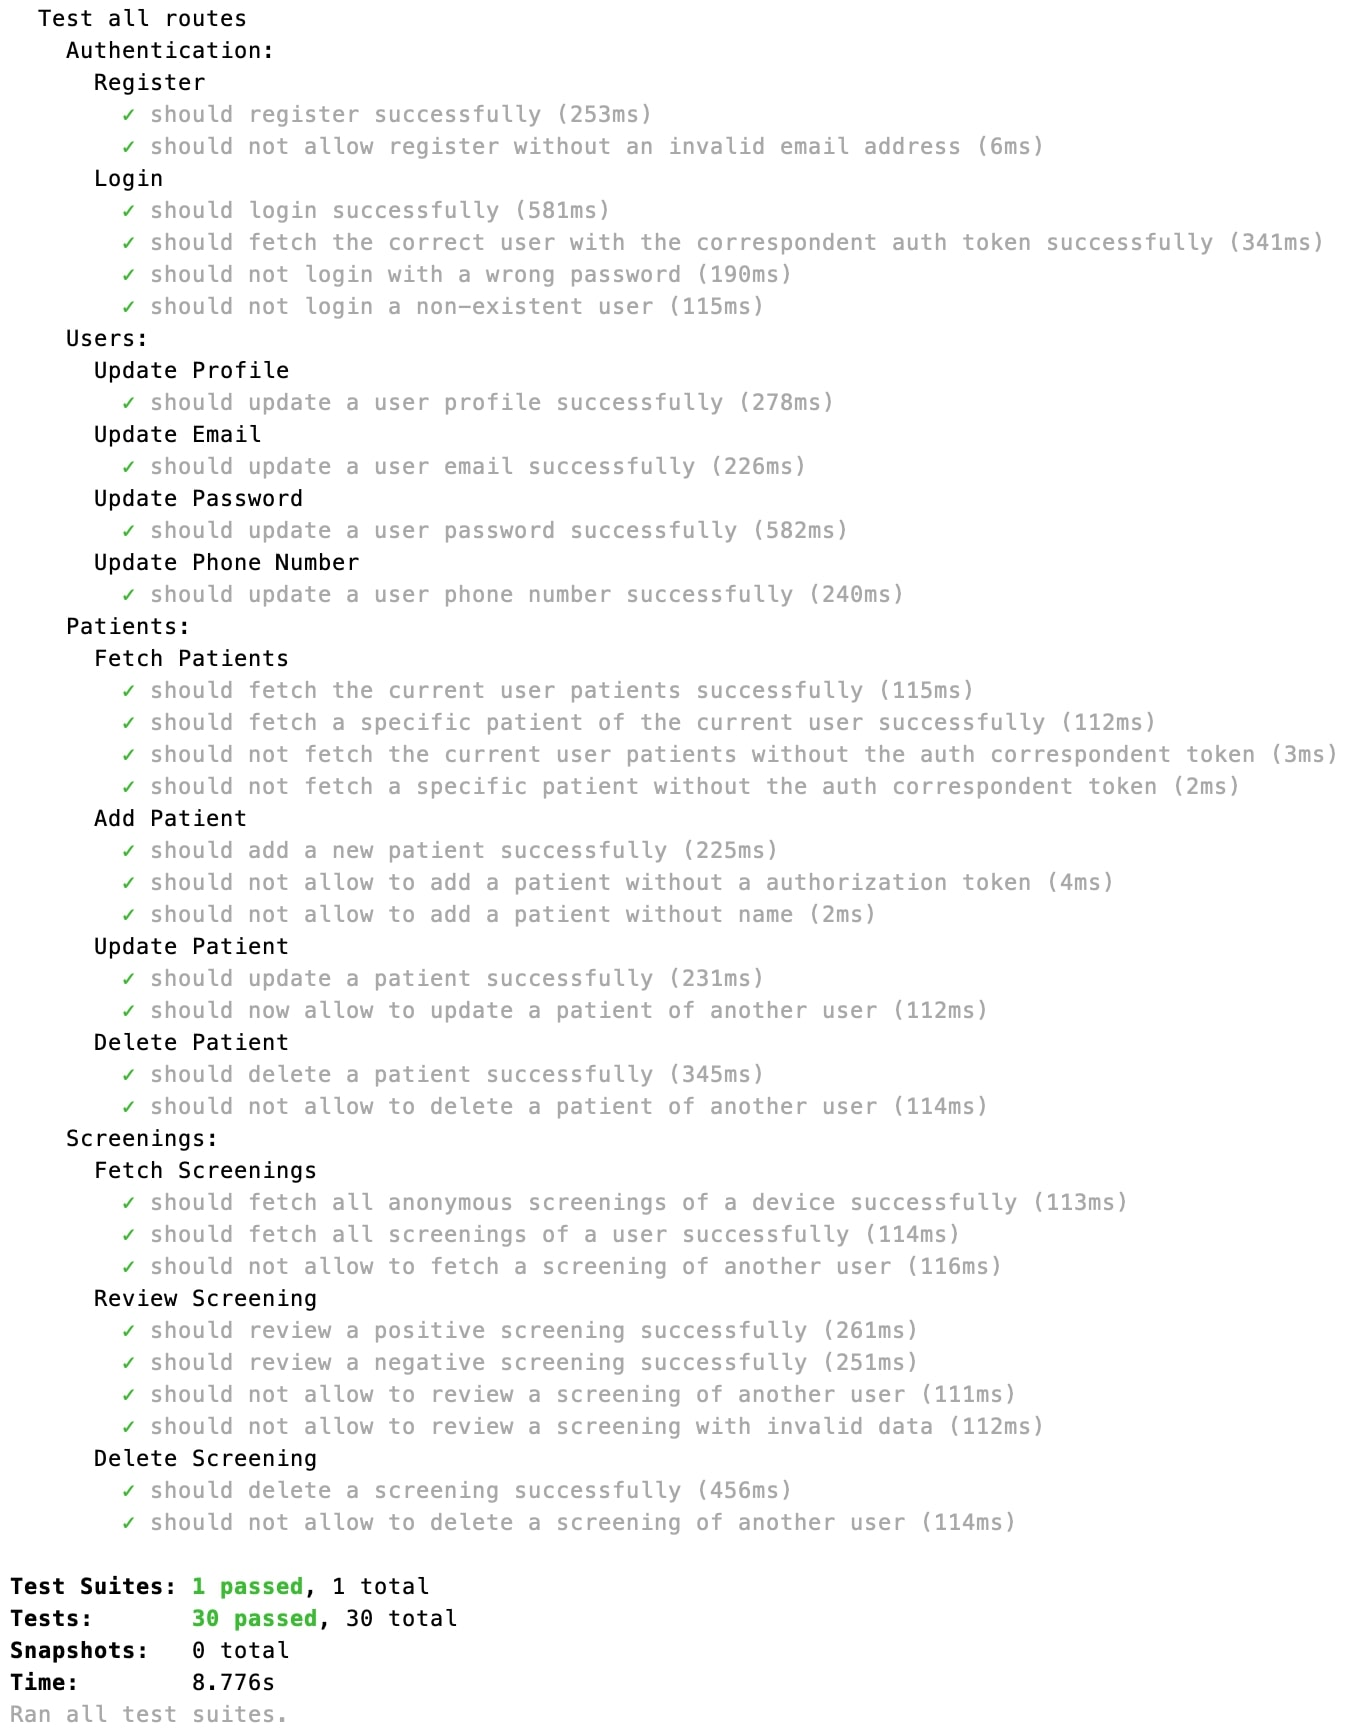
\includegraphics[width=1.0\linewidth]{pesti-report/images/unit-tests.jpg}
	\caption{Unit tests}
	\label{fig:unit-tests}
\end{figure}
\\

\section{Releases and deployment}

During our first face-to-face meeting in Belgium we decided that we would release and deploy the system as a whole and not the specific components (web client, mobile client and API). So instead of releasing by component we would release by feature, where we would develop the back-end and the front-end simultaneously.
\\ \\
We didn't agree on a fixed schedule of releases, so we would be releasing and documenting the changes every time we would feel that we had a good amount of issues delivered on that release. During our development time, we released three private alpha versions and a public open-source beta version. Below is our release management change-log:

\subsection{Version 0.1.0}

We released the alpha version 0.1.0 on 21 March 2020 with the following features:

\begin{itemize}

\item
Register
\item
Login
\item
Logout
\item
View the user profile
\item
Diagnose a screening
\item
View the screenings list
\item
View the details of a specific screening
\item
Add a patient
\item
View the patients list
\item
View the details of a specific patient
\item
View the about page
\item
View the privacy policy page

\end{itemize}

\subsection{Version 0.2.0}

Our second deployment, the alpha version 0.2.0 was released on the 8th of April of the same year with the following changes:

\begin{itemize}

\item
Edit the user profile (name, city, country and bio)
\item
Edit the user password
\item
Edit the user phone number
\item
Edit the user email address
\item
Reference a patient when diagnosing a screening
\item
View the output image of a screening
\item
Edit a patient details (name, sex and year of birth)
\item
View breadcrumbs for better navigation
\item
View the terms and conditions page
\item
View the cookie banner
\item
Multiple bug fixes

\end{itemize}

\subsection{Version 0.3.0}

Our third and last alpha deployment, the alpha version 0.3.0 was released on the 10 June 2020 with the following changes:

\begin{itemize}

\item
Send location data (latitude and longitude) when diagnosing a screening
\item
Properly view the diagnosis result of a screening
\item
Properly validate all input fields
\item
Refactored the style of the application
\item
Add contact page and form
\item
Multiple bug fixes

\end{itemize}

\subsection{Version 1.0.0}

Two days after our third release, on 12 June 2020, we released or first beta version 1.0.0, with some small bug fixes and deployed all our code on GitHub public as open source software using the MIT license.

